\documentclass[10pt,letterpaper]{article}

% ============================================================================
% Nature / bioRxiv Preprint Layout (XeLaTeX / Tectonic)
% Single unified Arial font matching all 5 Fignimble vector figures
% Strictly black typography: color appears exclusively in figures
% Zero gray text boxes
% ============================================================================
\usepackage[letterpaper,left=0.82in,right=0.82in,top=0.74in,bottom=0.74in,headheight=19pt]{geometry}
\usepackage{fontspec}
\usepackage{amsmath,amssymb}
\usepackage{graphicx}
\usepackage{booktabs}
\usepackage{array}
\usepackage{tabularx}
\usepackage{xcolor}
\usepackage{caption}
\usepackage{titlesec}
\usepackage{fancyhdr}
\usepackage{lastpage}
\usepackage{enumitem}
\usepackage{microtype}
\usepackage[hidelinks]{hyperref}
\urlstyle{same}

% Single cohesive font family (Arial) across text and figures (Nature convention)
\setmainfont{Arial}[
  Scale=0.95,
  BoldFont={Arial Bold},
  ItalicFont={Arial Italic},
  BoldItalicFont={Arial Bold Italic}
]
\setsansfont{Arial}[Scale=0.95]
\setmonofont{Arial}[Scale=0.95]

% Clean journal reading rhythm and tight float-text co-placement
\linespread{1.11}
\setlength{\parindent}{0pt}
\setlength{\parskip}{4.4pt}
\setlength{\emergencystretch}{3em}
\renewcommand{\topfraction}{0.88}
\renewcommand{\bottomfraction}{0.80}
\renewcommand{\textfraction}{0.08}
\renewcommand{\floatpagefraction}{0.80}

% Monochrome black text throughout; subtle neutral gray only for hairlines
\definecolor{RuleGray}{HTML}{BDBDBD}
\color{black}

% Section and subsection headings: pure black, declarative, clean hierarchy
\titleformat{\section}
  {\fontsize{12.2}{15}\selectfont\bfseries\color{black}}
  {\thesection.}{0.5em}{}
  [\vspace{-3pt}\textcolor{RuleGray}{\rule{\textwidth}{0.5pt}}]
\titlespacing*{\section}{0pt}{14pt}{6pt}

\titleformat{\subsection}
  {\fontsize{10.8}{13.5}\selectfont\bfseries\color{black}}
  {\thesubsection}{0.55em}{}
  \titlespacing*{\subsection}{0pt}{10pt}{3.5pt}

% Nature-style captions (pure black Arial, bold label, ragged right)
\captionsetup{
  font={small,sf,color=black},
  labelfont={bf,color=black},
  labelsep=period,
  skip=6pt,
  justification=raggedright,
  singlelinecheck=false
}

% Running headers and footers (pure black)
\pagestyle{fancy}
\fancyhf{}
\renewcommand{\headrulewidth}{0.4pt}
\renewcommand{\headrule}{\hbox to\headwidth{\color{RuleGray}\leaders\hrule height \headrulewidth\hfill}}
\fancyhead[L]{\footnotesize\color{black}Koppikar (2026) \textbar\ A 600-My +2 dual-coding gene family inside human \textit{PRRC2A} and \textit{PRRC2B}}
\fancyhead[R]{\footnotesize\color{black}Preprint}
\fancyfoot[C]{\footnotesize\color{black}\thepage\ / \pageref{LastPage}}

\fancypagestyle{firstpage}{
  \fancyhf{}
  \renewcommand{\headrulewidth}{0pt}
  \fancyfoot[C]{\footnotesize\color{black}\thepage\ / \pageref{LastPage}}
}

% Semantic helpers (same Arial body font throughout; Nature superscript citations)
\newcommand{\spname}[1]{\textit{#1}}
\newcommand{\gene}[1]{\textit{#1}}
\newcommand{\refsup}[1]{\textsuperscript{#1}}

\begin{document}
\thispagestyle{firstpage}

% ============================================================================
% TITLE BLOCK
% ============================================================================
\noindent{\fontsize{15.0}{18.5}\selectfont\bfseries\color{black}\raggedright
An Uncharacterized 600-Million-Year-Old +2 Dual-Coding Gene Family Embedded Inside the Human Leaky-Scanning Regulators \gene{PRRC2A} and \gene{PRRC2B}\par}
\vspace{5pt}

\noindent{\normalsize\color{black}
Pratik Koppikar\textsuperscript{1,*}\\[2pt]
{\small\color{black}
\textsuperscript{1}University of Cambridge, Cambridge, United Kingdom \;\textbar\; \textsuperscript{*}Correspondence: \href{mailto:psk34@cam.ac.uk}{psk34@cam.ac.uk} \;\textbar\; ORCID: \href{https://orcid.org/0000-0001-5089-5584}{0000-0001-5089-5584}\\
Code Availability: \url{https://github.com/koppikarp/prrc2-plus2-dualcoding}\par
}}
\vspace{2pt}
\noindent{\color{RuleGray}\rule{\textwidth}{0.7pt}}
\vspace{4pt}

% ============================================================================
% ABSTRACT
% ============================================================================
\noindent{\fontsize{11.0}{13.8}\selectfont\bfseries\color{black} Abstract}
\vspace{2pt}

True dual-coding exons, in which two unrelated proteins are translated from overlapping out-of-frame coding sequences on the same mRNA, are exceptionally rare in humans. Through a frame-agnostic screen of 23,183 canonical human protein-coding genes across 100 vertebrates, we identify a deeply conserved +2 dual-coding paralog family embedded across coding exons 2--6 of the translation-initiation regulators \gene{PRRC2A} (chr6 MHC class III) and \gene{PRRC2B} (chr9). These overlapping proteins---\gene{alt-PRRC2A} (130 aa) and \gene{alt-PRRC2B} (142 aa)---occupy the unstructured N-terminal ``BAT2'' domain (InterPro IPR009738) of unknown function. Although HAVANA/GENCODE quietly added unnamed stubs in May 2022 (\texttt{ENSG00000289282}/UniProt \texttt{A0A8I5QKQ9}, protein-level evidence via PeptideAtlas; \texttt{ENSG00000288841}/\texttt{A0A8I5KXM2}), both lack HGNC symbols, RefSeq/NCBI/GTEx entries, Pfam/InterPro domains, and any published characterization, with Ensembl Compara listing only human and mouse.

Tracing \gene{PRRC2}/\gene{nocte} across animals shows that the +2 frame is absent in protostomes (\spname{Drosophila} \gene{nocte}, 4 stops) but arose at the base of deuterostomes $\sim 580$\,Mya (0 stops in acorn worm and sea urchin), locked its \texttt{SAAG[I/V]AA[T/A]AGF[T/A]} and \texttt{VVWARTKPPP} motifs through amphioxus and lamprey, and survived vertebrate whole-genome duplications in \gene{PRRC2A} and \gene{PRRC2B} while pseudogenizing in \gene{PRRC2C} before jawed vertebrates ($> 465$\,Mya; 10--13 stops in human and shark \gene{PRRC2C}). Using \gene{PRRC2C} as a built-in paralog negative control, orthogonal vertebrate tests demonstrate +2 purifying selection: strict non-stop-risk 4D synonymous identity surges inside the overlap (\gene{PRRC2A} 0.874 vs.\ 0.613, $P = 2.38 \times 10^{-7}$; \gene{PRRC2B} 0.868 vs.\ 0.570, $P = 1.49 \times 10^{-8}$; both $P \le 3.74 \times 10^{-6}$ vs.\ \gene{PRRC2C}), only Frame +2 collapses to near-zero stops (0.05--0.08 vs.\ 6.0--6.2 expected under a within-gene flanking-codon synonymous null, and significantly below all four other alternative frames within the same DNA, 1.0--7.5 stops, max $P \le 1.51 \times 10^{-5}$; 94/98 \gene{PRRC2B} and 74/84 \gene{PRRC2A} vertebrates stop-free vs.\ 0/85 in \gene{PRRC2C}), and the overlapping +2 residue(s) touched by Frame-0-divergent mutations stay conserved at 28.8\% and 53.5\% vs.\ 8.3\% in \gene{PRRC2C} ($P \le 3.14 \times 10^{-5}$).

Across 807,162 human exomes and genomes in gnomAD v4.1 (QC-PASS variants), Frame-0-synonymous / Frame-+2-nonsense mutations are severely depleted: 0/35 non-CpG sites are observed across pooled \gene{PRRC2A}+\gene{PRRC2B} (0.0\%, $\text{AC} = 0$) versus 94/533 non-stop sites (17.6\%, $\text{AC} = 62,444$; Fisher $P = 1.43 \times 10^{-3}$), alongside CpG depletion (2/7 vs.\ 25/28, $P = 3.04 \times 10^{-3}$; three-stratum exact hypergeometric CMH $\text{OR} = 0.019$, one-sided $P = 9.06 \times 10^{-6}$, two-sided $P = 1.28 \times 10^{-5}$), replicating independently in \gene{PRRC2A} ($P = 1.15 \times 10^{-3}$) and \gene{PRRC2B} ($P = 1.10 \times 10^{-2}$) while vanishing in \gene{PRRC2C} ($\text{OR} = 0.763$, $P = 0.490$). GTEx v2 junctions ($\sim 19,000$ samples) rule out alternative splicing ($\sim 99\%$ canonical across coding exons 1--6), and GENCODE Ribo-seq reveals an ancestral +2 upstream overlapping ORF (\texttt{c6riboseqorf41}/\texttt{c9riboseqorf98}) at $-16$\,nt that crosses a 100\%-conserved suboptimal $+4$\,T Frame-0 start (\texttt{G/ATG/T}) and terminates exactly 183\,nt upstream of the 100\%-conserved optimal \texttt{[A/G]NNATGG} start of \gene{alt-PRRC2A/B}---defining a candidate \gene{ATF4}-like reinitiation circuit inside the leaky-scanning regulators themselves. We re-annotate 23 ClinVar variants and design genomically audited single-nucleotide knockout switches---including bystander-free \texttt{SpCas9-NG}/\texttt{SpRY}-CBE \texttt{Q4*} switches and canonical \texttt{NGG}-PAM \texttt{Q96*}/\texttt{Q97*} switches---to ablate either +2 protein without altering Frame-0 \gene{PRRC2A/B}.

\vspace{6pt}
\begin{figure}[!htbp]
  \centering
  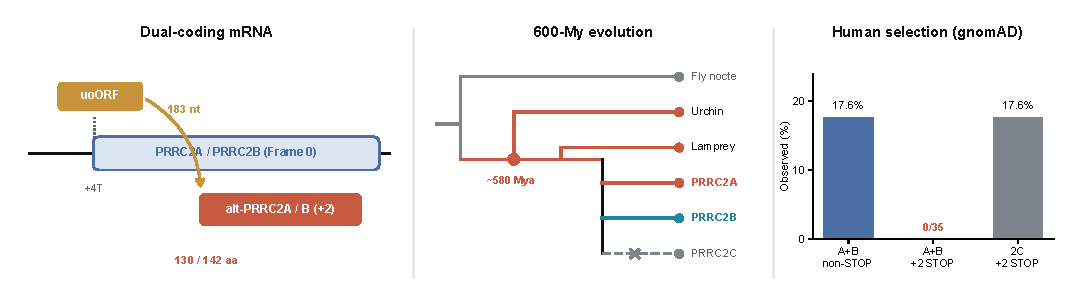
\includegraphics[width=\textwidth]{figures/rendered/graphical_abstract.pdf}
  \caption*{\textbf{Graphical Abstract.} Human \gene{PRRC2A} and \gene{PRRC2B} share an ancestral +2 upstream overlapping ORF (\texttt{uoORF}) and exact 183\,nt reinitiation spacer bypassing the suboptimal $+4$\,T Frame-0 start (\texttt{G/ATG/T}) to translate a 130/142-aa dual-coding protein (\gene{alt-PRRC2A/B}) born in early deuterostomes ($\sim 580$\,Mya), lost in \gene{PRRC2C}, and actively purged of Frame-0-silent / Frame-+2-nonsense mutations across 807,162 human exomes and genomes (0/35 QC-PASS non-CpG sites observed vs.\ 17.6\% in non-stop sites and \gene{PRRC2C}).}
\end{figure}

% ============================================================================
% 1. INTRODUCTION
% ============================================================================
\section{Introduction}

In viruses and compact prokaryotic genomes, overlapping reading frames are a well-established strategy for packing additional regulatory proteins into limited sequence space\refsup{1,2}. In the human genome, by contrast, bona fide dual-coding exons---where two unrelated amino-acid sequences are translated from overlapping reading frames of the exact same mature mRNA---are vanishingly rare. Fewer than two dozen human dual-coding loci have been experimentally validated or definitively proven to evolve under dual-frame purifying selection, including classic examples such as \gene{CDKN2A} (\texttt{p16INK4a}/\texttt{p14ARF})\refsup{3}, \gene{GNAS} (\texttt{XL}$\alpha$\texttt{s}/\texttt{ALEX})\refsup{4}, \gene{ATXN1} (\texttt{Alt-ATXN1})\refsup{5}, \gene{POLG} (\texttt{POLGARF})\refsup{6}, \gene{FUS} (\texttt{altFUS})\refsup{7}, and \gene{RPL36} (\texttt{alt-RPL36})\refsup{8}. Because genome annotation pipelines and clinical variant-effect predictors routinely assume one reading frame per coding exon, uncharacterized dual-coding proteins remain invisible to standard comparative genomics, transcriptomics, and clinical variant interpretation\refsup{9,10}.

The human \gene{PRRC2} family---comprising \gene{PRRC2A} (historically \gene{BAT2}, located in the chromosome 6 MHC class III region), \gene{PRRC2B} (chromosome 9), and \gene{PRRC2C} (chromosome 1)---encodes three large ($\sim 2,150$--$2,900$\,aa), predominantly intrinsically disordered RNA-binding proteins that localize to stress granules and are each strongly intolerant to loss-of-function variation in humans\refsup{11--15}. Over the past several years, independent biochemical and ribosome-profiling studies have converged on a central cellular role for the \gene{PRRC2} family: \gene{PRRC2A}, \gene{PRRC2B}, and \gene{PRRC2C} associate directly with the eIF3 translation initiation complex and eIF4G2 (DAP5) to promote ribosomal leaky scanning past inhibitory upstream open reading frames (uORFs) and overlapping uORFs (uoORFs), thereby governing the translation of proliferation, cell-cycle, and neurodevelopmental mRNAs\refsup{11--13}. In addition, \gene{PRRC2A} has been implicated as an $m^6\text{A}$-binding regulator of oligodendroglial specification and myelination\refsup{16}, while the invertebrate ortholog \gene{nocte} controls sensory temperature entrainment of the circadian clock in \spname{Drosophila}\refsup{17}.

Despite intense interest in the \gene{PRRC2} family, its N-terminal ``BAT2'' domain (InterPro IPR009738, spanning roughly the first 200 amino acids of \gene{PRRC2A}, \gene{PRRC2B}, and \gene{PRRC2C}) has remained a structural and functional enigma. A February 2026 comparative study dedicated to the human \gene{PRRC2} paralogs explicitly noted that BAT2 is ``a $\sim 200$-residue-long domain that lacks a stable structure with no known function,'' while finding unexplained compositional divergence between the BAT2 region of \gene{PRRC2C} and those of \gene{PRRC2A} and \gene{PRRC2B}\refsup{13}.

Here, we resolve this puzzle by showing that coding exons 2--6 of the BAT2 region of \gene{PRRC2A} and \gene{PRRC2B} are dual-coding, housing a 600-million-year-old +2 reading frame (\gene{alt-PRRC2A}, 130 aa; \gene{alt-PRRC2B}, 142 aa) that originated in early deuterostomes and was lost specifically in \gene{PRRC2C} before the origin of jawed vertebrates. By combining 100-vertebrate comparative genomics, within-gene synonymous null modeling, mutation-class-stratified purifying selection across 807,162 human exomes and genomes in gnomAD v4.1\refsup{14,15}, GTEx v2 splice-junction profiling\refsup{18}, and GENCODE Phase I ribosome-profiling annotations\refsup{19}, we establish that \gene{alt-PRRC2A} and \gene{alt-PRRC2B} are under active protein-level purifying selection in living humans, uncover a candidate uoORF reinitiation architecture shared across the \gene{PRRC2} transcripts themselves, re-annotate 23 ClinVar clinical variants\refsup{20}, and design genomically audited base- and prime-editing knockout switches for immediate experimental dissection.

% ============================================================================
% 2. RESULTS
% ============================================================================
\section{Results}

\subsection{A genome-wide 100-vertebrate screen uncovers a conserved +2 dual-coding family inside \gene{PRRC2A} and \gene{PRRC2B}}

To search systematically for uncharacterized dual-coding exons in the human genome without relying on existing gene annotations, we scanned all 23,183 canonical human protein-coding transcripts (UCSC \texttt{knownCanonical}, hg38) across 100 vertebrate alignments for long, stop-free internal reading frames (+1 or +2) showing sharp localized spikes in fourfold degenerate (4D) synonymous-site conservation relative to each transcript's own flanking coding sequence. After filtering out single-exon artifacts, readthrough transcripts, and previously annotated overlapping loci, two paralogous loci stood out at the top of the multi-exon dual-coding rankings: a 142-codon +2 open reading frame embedded across coding exons 2--6 of \gene{PRRC2B} (chromosome 9, \texttt{ENST00000357304.8}, CDS nucleotides 257--683; raw rank 2 genome-wide) and its 130-codon homologous +2 open reading frame across coding exons 2--6 of \gene{PRRC2A} (chromosome 6 MHC class III, \texttt{ENST00000376033.3}, CDS nucleotides 254--644; raw rank 29 via \texttt{ENST00000454306.6}; Fig.~\ref{fig:fig1}a).

\begin{figure}[!htbp]
  \centering
  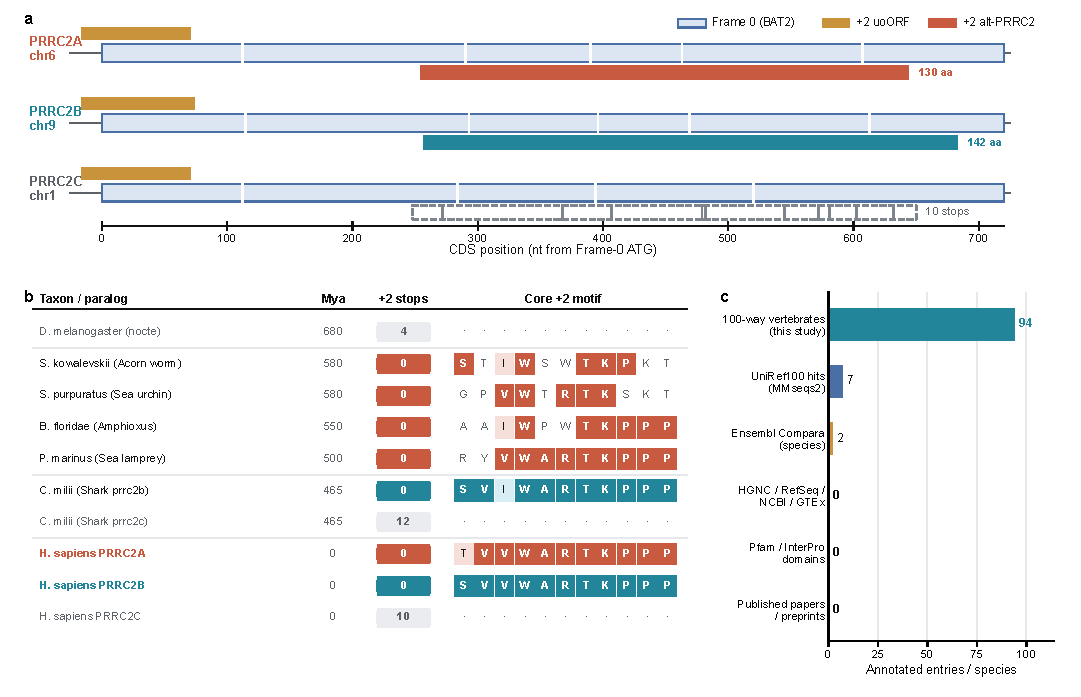
\includegraphics[width=\textwidth]{figures/rendered/fig1.pdf}
  \caption{\textbf{Genomic architecture, 600-million-year deuterostome origin, and database blind spot of \gene{alt-PRRC2A} and \gene{alt-PRRC2B}.} \textbf{a}, To-scale schematic of coding exons 1--6 (CDS nucleotides 0--720) of human \gene{PRRC2A} (chr6), \gene{PRRC2B} (chr9), and the pseudogenized paralog \gene{PRRC2C} (chr1). Frame-0 BAT2 coding exons are shown in light slate blue (white vertical ticks denote exact hg38 exon junctions), the conserved +2 upstream overlapping ORF (\texttt{uoORF}, starting at $-16$\,nt) in ochre, and the embedded +2 reading frame (\gene{alt-PRRC2A}, 130 aa, terracotta; \gene{alt-PRRC2B}, 142 aa, petrol teal; pseudogenized \gene{PRRC2C} bearing all 10 exact internal stop ticks, dashed gray). \textbf{b}, Evolutionary emergence and conservation across ten representative animal lineages spanning 680 million years, showing divergence time (Mya), internal +2 stop-codon counts across the homologous core, and the aligned 11-residue C-terminal \texttt{SVVWARTKPPP} signature motif (solid colored tiles indicate exact matches to the consensus; light tiles indicate biochemically conservative substitutions). \textbf{c}, Database annotation gap comparing the 94 vertebrate orthologs recovered for \gene{alt-PRRC2B} in our 100-way alignment against current counts in UniRef100 (7 MMseqs2 hits), Ensembl Compara (2 species: human and mouse), HGNC/RefSeq/NCBI Gene/GTEx (0), Pfam/InterPro (0), and published literature or preprints (0).}
  \label{fig:fig1}
\end{figure}

Remarkably, both embedded polypeptides (\gene{alt-PRRC2A} and \gene{alt-PRRC2B}) span the exact unstructured N-terminal BAT2 domain (InterPro IPR009738) of their host proteins (Frame-0 codons 85--214 in \gene{PRRC2A}; codons 86--227 in \gene{PRRC2B}), sharing 59\% amino-acid identity across their aligned 129-residue core (76/129; 53\% overall including the 12-residue C-terminal extension of \gene{alt-PRRC2B}) across three sharply conserved sequence blocks: an N-terminal hydrophobic/alanine-rich tract (\texttt{SAAG[I/V]AA[T/A]AGF[T/A]}), a central basic/aliphatic core (\texttt{KG[I/L]KPTV[T/I][I/L]LSRGIS}), and a C-terminal proline-capped motif (\texttt{WR[P/A]GQG...VVWARTKPPP}). By contrast, the homologous coding exon 2--5 span of the third human paralog, \gene{PRRC2C} (chromosome 1, \texttt{ENST00000338920.8}, CDS nucleotides 248--650), is riddled with 10 in-frame stop codons in Frame +2 (Fig.~\ref{fig:fig1}a), providing an ideal built-in evolutionary negative control.

Auditing public sequence and literature databases revealed a striking annotation blind spot (Fig.~\ref{fig:fig1}c). On May 25, 2022, HAVANA/GENCODE quietly instantiated two unnamed ``novel protein'' stub records corresponding precisely to these +2 ORFs---\texttt{ENSG00000289282} (\texttt{ENST00000687518.1}, UniProt \texttt{A0A8I5QKQ9}, 130 aa) inside \gene{PRRC2A} and \texttt{ENSG00000288841} (\texttt{ENST00000691540.1}, UniProt \texttt{A0A8I5KXM2}, 142 aa) inside \gene{PRRC2B}\refsup{21,22}. Crucially, UniProt assigns \texttt{A0A8I5QKQ9} a Protein Existence score of \texttt{PE=1} (``Evidence at protein level'') based on mass-spectrometry peptide detection in PeptideAtlas\refsup{23,24}, confirming physical translation in human samples, whereas \texttt{A0A8I5KXM2} remains \texttt{PE=4} (``Predicted''). Yet neither locus has ever been named or investigated: both have zero HGNC gene symbols, zero NCBI Gene or RefSeq accessions, zero GTEx expression entries, zero Pfam or InterPro domain classifications, and zero mentions across PubMed, PubMed Central, Europe PMC, or bioRxiv. Ensembl Compara records orthologs in only two species (human and mouse, \texttt{ENSMUSG00000144229}), and searching \gene{alt-PRRC2B} against the entire UniRef100 database with MMseqs2 returned only 7 hits---compared to 94 stop-free vertebrate orthologs in our 100-way genomic alignment alone.

\subsection{The +2 reading frame originated at the base of deuterostomes $\sim 580$ million years ago and pseudogenized in \gene{PRRC2C} before jawed vertebrates}

To determine when the +2 reading frame arose and why \gene{PRRC2C} lacks it, we retrieved full-length \gene{PRRC2}/\gene{nocte} coding sequences spanning protostomes, basal deuterostomes, jawless vertebrates, cartilaginous fish, and mammals, and translated their homologous BAT2 regions in all three forward reading frames (Fig.~\ref{fig:fig1}b).

In the protostome outgroup \spname{Drosophila melanogaster} (\gene{nocte}, \texttt{NP\_001245614.1}, diverged $\sim 680$ million years ago [Mya]), the N-terminal BAT2 domain is well conserved in Frame 0, but both Frame +1 and Frame +2 are disrupted by 4 internal stop codons with zero homology to \gene{alt-PRRC2}. Immediately across the protostome--deuterostome boundary ($\sim 580$\,Mya), however, the +2 reading frame snaps open: both the hemichordate acorn worm (\spname{Saccoglossus kowalevskii}, \texttt{XP\_077866102.1}) and the echinoderm sea urchin (\spname{Strongylocentrotus purpuratus}, \texttt{XP\_030852947.1}) contain 0 internal stop codons in Frame +2 (versus 3 and 5 stops in Frame +1 across the homologous core) and already encode the N-terminal \texttt{MG[F/I]RR} initiator and proto-C-terminal \texttt{W[S/T][W/R]TK} motif (Fig.~\ref{fig:fig1}b). In the cephalochordate amphioxus (\spname{Branchiostoma floridae}, \texttt{XP\_035683835.1}, $\sim 550$\,Mya), the +2 frame remains stop-free and locks in both the alanine-rich tract (\texttt{SAAGTAAAAGFT}) and the proline-capped C-terminus (\texttt{AAIWPWTKPPP}). By the jawless vertebrate sea lamprey (\spname{Petromyzon marinus}, \texttt{XP\_032802661.2}, $\sim 500$\,Mya), the +2 protein has assembled nearly its complete modern architecture (\texttt{AAGVAAAAGFISICR...RYVWARTKPPPTECKQLA*}).

Following the two rounds of early vertebrate whole-genome duplication (2R WGD) that split ancestral \gene{PRRC2} into \gene{PRRC2A}, \gene{PRRC2B}, and \gene{PRRC2C}, the fate of the +2 frame diverged cleanly before the emergence of jawed vertebrates. In the cartilaginous elephant shark (\spname{Callorhinchus milii}, $\sim 465$\,Mya), \gene{prrc2b} (\texttt{XM\_042337680.1}) retains a 100\% intact, stop-free +2 ORF (0 stops in +2 versus 5 in +1 across the homologous core) with every major human motif conserved (\texttt{MGKQAGAARAKEFRCVSSSAAGVAVAIGYA...SRGIS...SVIWARTKPPP}), whereas elephant shark \gene{prrc2c} (\texttt{XM\_042335521.1}) is already pseudogenized in Frame +2 with 13 internal stop codons (\texttt{MGH*TRTA*RREQ*Y}). We also audited rare ray-finned fish UniProt entries that appear to fuse BAT2 in-frame with \gene{alt-PRRC2} (such as sterlet \texttt{A0A444UTE8}/\texttt{RXM91444.1} and marine medaka \texttt{A0A3B3D8N8}/\texttt{ENSOMET00000004379}); exon-structure inspection showed that these represent automated gene-model frameshifts or exon-skipping artifacts (e.g., a 2-exon truncated model with a 115\,nt Exon 1 in medaka) rather than ancestral single-chain fusions. Together, these data place the origin of \gene{alt-PRRC2} at the dawn of deuterostomes ($\sim 580$\,Mya) and its paralog-specific loss in \gene{PRRC2C} prior to 465\,Mya.

\subsection{Vertebrate synonymous-site conservation, frame-specific stop purging, and +2 amino-acid preservation demonstrate protein-level purifying selection}

An extended alternative reading frame could in principle survive passively if local nucleotide composition disfavors stop codons or if Frame-0 exons harbor conserved RNA elements. To separate true protein-level purifying selection in Frame +2 from compositional or cis-regulatory confounders, we performed three orthogonal comparative tests across a non-redundant 32-vertebrate reference panel spanning primates to teleost fish (Panel-32), benchmarking \gene{PRRC2A} and \gene{PRRC2B} directly against their pseudogenized paralog \gene{PRRC2C} (Fig.~\ref{fig:fig2}).

\begin{figure}[!htbp]
  \centering
  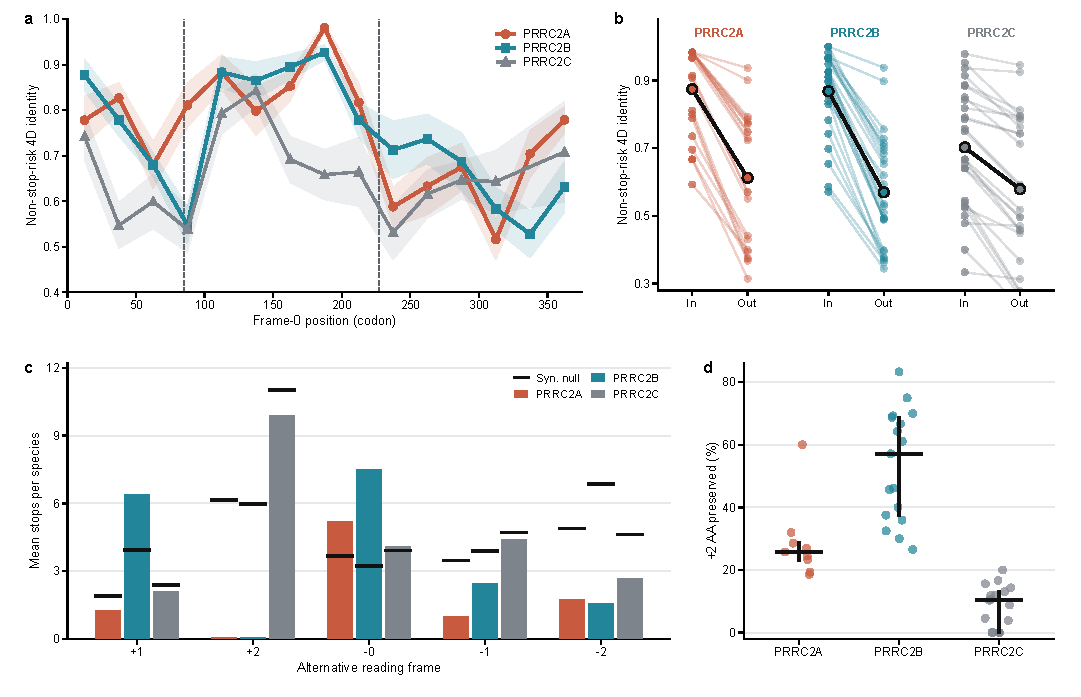
\includegraphics[width=\textwidth]{figures/rendered/fig2.pdf}
  \caption{\textbf{Orthogonal vertebrate signatures of purifying selection acting specifically on Frame +2 of \gene{PRRC2A} and \gene{PRRC2B}.} \textbf{a}, Sliding-window (25-codon bins, codons 0--375) strict non-stop-risk fourfold degenerate (4D) synonymous identity (mean $\pm 1$ species s.e.\ across Panel-32 vertebrates) for \gene{PRRC2A} (terracotta, $n = 22$ species), \gene{PRRC2B} (petrol teal, $n = 26$), and the pseudogenized paralog control \gene{PRRC2C} (gray, $n = 26$). Vertical dashed lines mark the +2 dual-coding span (codons 85--227). \textbf{b}, Paired per-species strict non-stop-risk 4D identity inside versus outside the +2 span (one paired slope per vertebrate species; bold lines and circles denote species means; \gene{PRRC2A} 22/22 and \gene{PRRC2B} 26/26 species inside $>$ outside, exact paired Wilcoxon $P = 2.38 \times 10^{-7}$ and $P = 1.49 \times 10^{-8}$; inside-minus-outside $\Delta$ significantly exceeds \gene{PRRC2C}, Mann--Whitney $P = 3.74 \times 10^{-6}$ and $P = 1.06 \times 10^{-7}$). \textbf{c}, Mean stop-codon counts per species across all five alternative reading frames ($+1$, $+2$, $-0$, $-1$, $-2$) within the homologous dual-coding span for \gene{PRRC2A} ($n = 22$), \gene{PRRC2B} ($n = 25$), and \gene{PRRC2C} ($n = 22$), compared against each species' own 300-replicate flanking-codon synonymous null expectation (horizontal black bars). Only Frame +2 collapses to near-zero stops (0.05 and 0.08 stops versus 6.15 and 5.97 expected in \gene{PRRC2A} and \gene{PRRC2B}, exact paired Wilcoxon $P = 2.38 \times 10^{-7}$ and $P = 2.98 \times 10^{-8}$), whereas \gene{PRRC2C} averages 9.91 stops. \textbf{d}, Fraction of Frame-0-divergent alignment columns at which the overlapping +2 amino acid(s) directly touched by the mutated nucleotide(s) remain identical to human across Panel-32 vertebrates (horizontal black bars = medians, vertical bars = IQR; \gene{PRRC2A} mean 28.8\%, \gene{PRRC2B} 53.5\% versus \gene{PRRC2C} 8.3\%; Mann--Whitney $P = 3.14 \times 10^{-5}$ and $P = 3.39 \times 10^{-7}$).}
  \label{fig:fig2}
\end{figure}

First, we measured synonymous-site conservation strictly at non-stop-risk fourfold degenerate (4D) codons in Frame 0: sites where the third nucleotide is completely synonymous in Frame 0, acts as the missense first codon position in Frame +2, and cannot generate a Frame +2 stop codon because the following Frame-0 codon does not begin with \texttt{AA}, \texttt{AG}, or \texttt{GA}. Across 25-codon sliding windows, strict non-stop-risk 4D identity climbs steeply across the +2 ORF in both \gene{PRRC2A} and \gene{PRRC2B}, peaking above 0.93--0.98 directly over the conserved \texttt{VVWARTKPPP} core (codons 175--200) before dropping sharply past the +2 stop codon (Fig.~\ref{fig:fig2}a). Collapsing to one inside and one outside measurement per vertebrate species (avoiding all-vs-all pairwise pseudoreplication), 22 of 22 \gene{PRRC2A} species (mean 0.874 inside versus 0.613 outside, $\Delta = +0.262$; exact one-sided paired Wilcoxon $P = 2.38 \times 10^{-7}$, two-sided $P = 4.77 \times 10^{-7}$) and 26 of 26 \gene{PRRC2B} species (mean 0.868 versus 0.570, $\Delta = +0.298$; exact one-sided $P = 1.49 \times 10^{-8}$, two-sided $P = 2.98 \times 10^{-8}$) showed massive synonymous constraint (Fig.~\ref{fig:fig2}b; all-4D codons gave virtually identical results: $+0.261$ and $+0.295$; collapsing further to 8 independent major vertebrate clades confirmed identical elevation in 8/8 clades: \gene{PRRC2A} $\Delta = +0.259$, \gene{PRRC2B} $\Delta = +0.289$, both exact paired Wilcoxon $P = 3.91 \times 10^{-3}$). Crucially, while the pseudogenized paralog \gene{PRRC2C} displays a modest regional baseline elevation across the same N-terminal exons (0.702 inside versus 0.579 outside, $\Delta = +0.123$, reflecting general 5'-proximal exon-junction constraint), direct between-paralog comparisons demonstrate that both \gene{PRRC2A} ($\Delta = +0.262$ versus $+0.123$; one-sided Mann--Whitney $U$ $P = 3.74 \times 10^{-6}$, two-sided $P = 7.47 \times 10^{-6}$) and \gene{PRRC2B} ($\Delta = +0.298$ versus $+0.123$; one-sided $P = 1.06 \times 10^{-7}$, two-sided $P = 2.12 \times 10^{-7}$) carry more than double the synonymous constraint of \gene{PRRC2C}, concentrated squarely over the +2 coding core (Fig.~\ref{fig:fig2}a,b).

Second, we quantified stop-codon depletion across all five alternative reading frames ($+1$, $+2$, $-0$, $-1$, $-2$) within the homologous dual-coding span and benchmarked every species against its own within-gene flanking-codon synonymous null (300 replicates per vertebrate, 1,000 replicates for human hg38, resampling Frame-0 synonymous codons inside the overlap strictly from each gene's own outside-overlap codon usage while preserving exact Frame-0 amino-acid sequence; Fig.~\ref{fig:fig2}c). In human hg38, Frame +2 contains 0 stops versus 7.59 expected in \gene{PRRC2A} and 0 versus 5.76 expected in \gene{PRRC2B}, compared with 10 observed versus 12.61 expected in \gene{PRRC2C}. Across Panel-32 vertebrates, only Frame +2 collapses to near-zero stops: a mean of 0.05 stops (median 0.0; 21/22 stop-free) versus 6.15 expected in \gene{PRRC2A} (exact one-sided paired Wilcoxon $P = 2.38 \times 10^{-7}$) and 0.08 stops (median 0.0; 23/25 stop-free) versus 5.97 expected in \gene{PRRC2B} ($P = 2.98 \times 10^{-8}$). Within the exact same DNA sequences, Frame +2 carries far fewer stops than every other alternative frame (which retain 1.00--7.52 stops on average) in both \gene{PRRC2A} (within-gene paired Wilcoxon max $P = 1.51 \times 10^{-5}$ against $+1$, $-0$, $-1$, and $-2$) and \gene{PRRC2B} (max $P = 1.35 \times 10^{-5}$). Although antisense frames $-1$ and $-2$ also lie below the flanking-codon null (a secondary effect of local GC3 composition shifts---e.g., \gene{PRRC2B} GC3 is 0.549 inside versus 0.656 outside---and antisense stop-shadowing, visible even in \gene{PRRC2C} Frame $-2$), a strict within-window codon-bag synonymous shuffle on hg38 holding exact local GC3 and codon composition constant confirms strong depletion in Frame +2 (\gene{PRRC2A} 0 vs.\ 4.61 expected, empirical $P = 2.00 \times 10^{-3}$; \gene{PRRC2B} 0 vs.\ 4.19, $P = 4.00 \times 10^{-3}$; \gene{PRRC2C} 10 vs.\ 12.49, $P = 0.135$). Expanding to the full 100-way alignment confirms that 74/84 covered \gene{PRRC2A} vertebrates (mean 0.12 stops; all 10 stop-bearing assemblies are single-stop non-mammalian vertebrates, with 100\% of covered mammals stop-free) and 94/98 \gene{PRRC2B} vertebrates (mean 0.04 stops; 100\% of covered mammals and birds stop-free) are completely stop-free in Frame +2, whereas 0/85 \gene{PRRC2C} vertebrates are stop-free (mean 9.69 stops; Frame +2 is the highest-stop frame of all five in \gene{PRRC2C}, within-gene $P = 1.00$).

Third, we tested whether Frame +2 actively protects its own amino-acid sequence even when the host BAT2 protein mutates. Restricting strictly to alignment columns inside the overlap where the Frame-0 amino acid diverged from human and evaluating the exact overlapping +2 codon(s) containing the mutated nucleotide position(s), the touched +2 amino acid(s) remained identical to human at 28.8\% of sites in \gene{PRRC2A} ($n = 9$ species with $\ge 10$ divergent sites) and 53.5\% in \gene{PRRC2B} ($n = 17$ species), compared with just 8.3\% in the pseudogenized control \gene{PRRC2C} ($n = 17$ species; a 3.5- to 6.4-fold enrichment; one-sided Mann--Whitney $U$ $P = 3.14 \times 10^{-5}$, two-sided $P = 6.28 \times 10^{-5}$ for \gene{PRRC2A}; one-sided $P = 3.39 \times 10^{-7}$, two-sided $P = 6.78 \times 10^{-7}$ for \gene{PRRC2B}; Fig.~\ref{fig:fig2}d; evaluating the upstream $[\text{prev\_b2}, \text{b0}, \text{b1}]$ +2 codon yields the same conclusion: 43.0\% and 60.0\% vs.\ 23.8\%, one-sided $P = 4.15 \times 10^{-5}$ and $P = 4.56 \times 10^{-7}$).

\subsection{Population variation across 807,162 human exomes and genomes demonstrates active purifying selection on \gene{alt-PRRC2A} and \gene{alt-PRRC2B} in living humans}

Deep vertebrate conservation alone cannot rule out the possibility that a dual-coding gene recently became dispensable in the human lineage. To test directly whether \gene{alt-PRRC2A} and \gene{alt-PRRC2B} remain under active purifying selection in contemporary human populations, we analyzed all quality-control-passing (QC-PASS) single-nucleotide variants (SNVs) across coding exons 2--6 of \gene{PRRC2A} and \gene{PRRC2B} and homologous coding exons 2--5 of \gene{PRRC2C} in gnomAD v4.1 (807,162 human exomes and genomes; 730,947 exomes and 76,215 genomes; 100\% hg38 reference-allele concordance across all 1,300 overlapping QC-PASS coding SNVs)\refsup{14,15}. Both host genes are strongly haploinsufficient in gnomAD v4.1 (\gene{PRRC2A}: $\text{pLI} = 1.00$, $\text{LOEUF} = 0.326$; \gene{PRRC2B}: $\text{pLI} = 1.00$, $\text{LOEUF} = 0.343$). To decouple selection on Frame +2 from selection on Frame 0---and to eliminate mutational-rate confounding between hypermutable CpG transitions, non-CpG transitions, and transversions---we enumerated every possible single-nucleotide substitution inside the +2 coding span, stratified all sites into three exact mutational classes (\texttt{CpG\_Ti}, \texttt{nonCpG\_Ti}, and \texttt{Tv}), and held the Frame-0 consequence strictly constant while comparing Frame +2 consequences (Fig.~\ref{fig:fig3}).

\begin{figure}[!htbp]
  \centering
  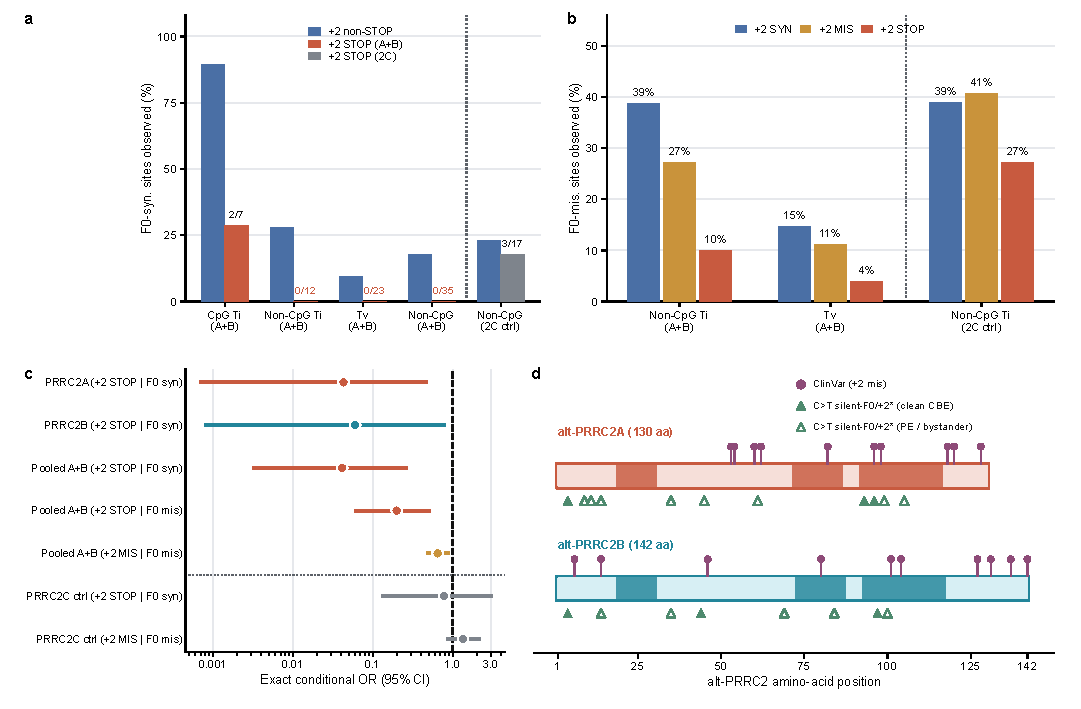
\includegraphics[width=\textwidth]{figures/rendered/fig3.pdf}
  \caption{\textbf{Active purifying selection on \gene{alt-PRRC2A} and \gene{alt-PRRC2B} across 807,162 human exomes and genomes in gnomAD v4.1 (QC-PASS) and clinical variant mapping.} \textbf{a}, Fraction of possible Frame-0-synonymous SNVs observed in gnomAD v4.1 stratified by mutational class (\texttt{CpG\_Ti}, \texttt{nonCpG\_Ti}, \texttt{Tv}, and combined \texttt{non-CpG}) for pooled \gene{PRRC2A} + \gene{PRRC2B} compared against the pseudogenized paralog negative control \gene{PRRC2C} (right of dotted line). Numbers above +2 STOP bars give exact observed/possible site counts: 0/12 non-CpG transitions, 0/23 transversions, 0/35 combined non-CpG sites (total allele count 0), and 2/7 CpG transitions (allele count 3) in \gene{PRRC2A}+\gene{PRRC2B}, versus 3/17 (17.6\%) in \gene{PRRC2C}. \textbf{b}, Ordered purifying-selection gradient among Frame-0-missense SNVs (\texttt{+2 SYN} $>$ \texttt{+2 MIS} $>$ \texttt{+2 STOP}) across non-CpG transitions and transversions in \gene{PRRC2A}+\gene{PRRC2B}, contrasted with the flat/unconstrained profile in \gene{PRRC2C}. \textbf{c}, Mutation-class-stratified exact conditional MLE odds ratios and exact conditional 95\% confidence intervals (derived from the convolved noncentral hypergeometric distribution without continuity hacks) across \gene{PRRC2A} alone, \gene{PRRC2B} alone, pooled \gene{PRRC2A}+\gene{PRRC2B}, and \gene{PRRC2C} control (vertical dashed line at $\text{OR} = 1.0$; every \gene{PRRC2A}, \gene{PRRC2B}, and pooled \gene{PRRC2A}+\gene{PRRC2B} 95\% CI lies strictly below 1.0). \textbf{d}, Domain-motif maps of \gene{alt-PRRC2A} (130 aa) and \gene{alt-PRRC2B} (142 aa) highlighting the three 500-My conserved sequence blocks (dark bands), all 23 ClinVar missense variants affecting Frame +2 (plum lollipops above), and \texttt{C>T} silent-Frame-0 / Frame-+2-nonsense switches (filled sage triangles: genomically bystander-free \texttt{SpCas9-NGG} or \texttt{SpCas9-NG}/\texttt{SpRY}-CBE sites; open sage triangles: \texttt{C>T} sites carrying Frame-0-missense bystanders or lacking an \texttt{NG}/\texttt{NGG} PAM, recommended for prime editing or \texttt{SpRY}-CBE).}
  \label{fig:fig3}
\end{figure}

Holding Frame 0 strictly synonymous (\texttt{F0 = syn}) yields the cleanest possible test of purifying selection on Frame +2, because every site in this comparison leaves the canonical \gene{PRRC2A} or \gene{PRRC2B} protein sequence 100\% unchanged (Fig.~\ref{fig:fig3}a). Across pooled \gene{PRRC2A} and \gene{PRRC2B}, zero of 35 possible non-CpG Frame-0-synonymous / Frame-+2-nonsense mutations are observed anywhere in 807,162 individuals (0/12 non-CpG transitions and 0/23 transversions; 0.0\%, total allele count $\text{AC} = 0$), compared with 94 of 533 non-stop Frame-0-synonymous sites (17.6\%, $\text{AC} = 62,444$; one-sided Fisher exact $P = 1.43 \times 10^{-3}$, two-sided $P = 1.96 \times 10^{-3}$; within non-CpG transitions alone: 0/12 versus 65/232 [28.0\%], one-sided $P = 0.0219$, two-sided $P = 0.0396$). Even at hypermutable CpG transitions---where 89.3\% (25/28, $\text{AC} = 476$) of non-stop Frame-0-synonymous sites are polymorphic in gnomAD v4.1---only 2 of 7 Frame-+2-nonsense sites are seen, at ultra-rare singleton/doubleton counts (28.6\%, total $\text{AC} = 3$; exact Fisher $P = 3.04 \times 10^{-3}$). Combining all three mutational strata with an exact hypergeometric Cochran--Mantel--Haenszel (CMH) test confirms severe depletion of Frame-0-silent / Frame-+2-nonsense variants (Mantel--Haenszel common $\text{OR} = 0.019$, exact conditional MLE $\text{OR} = 0.041$ [95\% CI 0.003--0.261], exact one-sided $P = 9.06 \times 10^{-6}$, exact two-sided $P = 1.28 \times 10^{-5}$; asymptotic CMH one-sided $P = 5.44 \times 10^{-5}$; excluding all $\pm 2$\,bp exon-boundary positions yields virtually identical results: 0/35 vs.\ 91/515, $\text{OR} = 0.019$, exact one-sided $P = 8.59 \times 10^{-6}$, two-sided $P = 1.23 \times 10^{-5}$).

Crucially, this human purifying selection is not driven by a single locus, nor does it reflect an artifact of the BAT2 exon sequence. Testing each paralog independently replicates the exact same depletion in both \gene{PRRC2A} alone (non-CpG 0/17 versus 42/257, CpG 1/5 versus 12/14; 3-stratum CMH $\text{OR} = 0.021$, exact MLE $0.043$ [95\% CI 0.001--0.458], exact one-sided $P = 1.15 \times 10^{-3}$, exact two-sided $P = 1.90 \times 10^{-3}$) and \gene{PRRC2B} alone (non-CpG 0/18 versus 52/276, Fisher one-sided $P = 0.0268$; 3-stratum CMH $\text{OR} = 0.017$, exact MLE $0.060$ [95\% CI 0.001--0.779], exact one-sided $P = 1.10 \times 10^{-2}$, exact two-sided $P = 1.76 \times 10^{-2}$; Fig.~\ref{fig:fig3}c). Conversely, running the exact same pipeline on the homologous exons of \gene{PRRC2C} yields a completely null result: 3 of 17 non-CpG Frame-0-synonymous / Frame-+2-nonsense sites are observed (17.6\%) versus 53 of 232 non-stop sites (22.8\%; Fisher one-sided $P = 0.442$, two-sided $P = 0.770$; 3-stratum CMH $\text{OR} = 0.763$, exact MLE $0.775$ [95\% CI 0.135--3.010], exact one-sided $P = 0.490$, exact two-sided $P = 1.00$; Fig.~\ref{fig:fig3}a,c).

Independent corroboration comes from holding Frame 0 missense (\texttt{F0 = mis}) and ordering variants by their Frame-+2 severity (\texttt{+2 = SYN} $>$ \texttt{+2 = MIS} $>$ \texttt{+2 = STOP}; Fig.~\ref{fig:fig3}b). In pooled \gene{PRRC2A} + \gene{PRRC2B}, variant observation rates drop monotonically across every stratum: among non-CpG transitions, 38.7\% (86/222, $\text{AC} = 1,639$) of \texttt{+2 = SYN} sites are observed, falling to 27.2\% (53/195, $\text{AC} = 321$) for \texttt{+2 = MIS} (one-sided Fisher $P = 8.17 \times 10^{-3}$) and 10.0\% (3/30, $\text{AC} = 4$) for \texttt{+2 = STOP} ($P = 9.85 \times 10^{-4}$); among transversions, rates drop from 14.8\% (43/291) to 11.2\% (99/883) to 4.0\% (2/50, $P = 0.0228$). Across all three mutational strata, exact CMH tests confirm strong purifying selection against both Frame-+2 missense mutations ($\text{OR} = 0.645$, exact MLE $0.647$ [95\% CI 0.486--0.864], exact one-sided $P = 1.47 \times 10^{-3}$, exact two-sided $P = 2.70 \times 10^{-3}$) and Frame-+2 nonsense mutations ($\text{OR} = 0.201$, exact MLE $0.199$ [95\% CI 0.061--0.510], exact one-sided $P = 5.34 \times 10^{-5}$, exact two-sided $P = 1.16 \times 10^{-4}$), whereas \gene{PRRC2C} again shows zero depletion for \texttt{+2 = MIS} ($\text{OR} = 1.355$, exact one-sided $P = 0.928$) or \texttt{+2 = STOP} ($\text{OR} = 0.510$, $P = 0.101$; Fig.~\ref{fig:fig3}b,c). Thus, both \gene{alt-PRRC2A} and \gene{alt-PRRC2B} are actively constrained against nonsense and missense mutations in the living human population.

\subsection{Constitutive splicing, 100\%-conserved Kozak asymmetry, and an ancestral +2 uoORF define a candidate reinitiation architecture in \gene{PRRC2A} and \gene{PRRC2B}}

How do scanning human ribosomes bypass the canonical Frame-0 start codon of \gene{PRRC2A} and \gene{PRRC2B} and reach an internal +2 \texttt{ATG} more than 250 nucleotides downstream? Two competing mechanisms could produce \gene{alt-PRRC2A/B}: either an alternative splice isoform excises the Frame-0 start codon to expose the +2 \texttt{ATG}, or translation initiates directly on the canonical full-length mRNA via leaky scanning and uoORF-mediated reinitiation\refsup{25--27}.

To test the splicing hypothesis directly across human tissues, we queried all local positive-strand splice junctions spanning coding exons 1--6 of \gene{PRRC2A} and \gene{PRRC2B} across $\sim 19,000$ human RNA-seq samples in GTEx v2 via Snaptron\refsup{18} (Fig.~\ref{fig:fig4}c). Both genes are constitutively spliced in the canonical reading frame across virtually all human tissues: the five canonical internal introns spanning coding exons 1--6 of \gene{PRRC2A} are supported by 1.12--1.52 million reads (mean 1.30 million) across 19,059--19,066 samples, whereas the most abundant alternative junction inside coding exons 1--6 (\texttt{chr6:31,622,902--31,624,260}, skipping coding exon 2) carries only 6,811 reads (0.52\% of mean canonical plus alternative reads; 0.45\% relative to flanking Intron 1--2), and the top upstream junction skipping coding exon 1 (\texttt{chr6:31,620,859--31,623,731}) carries 7,369 reads (0.56\%; $> 99.4\%$ canonical). Likewise, the five canonical internal introns spanning coding exons 1--6 of \gene{PRRC2B} carry 319,296--657,965 reads (mean 534,897) across 18,703--18,983 samples versus 5,655 reads (1.05\% of mean canonical plus alternative reads; 0.87\% relative to flanking Intron 3--4) for the top internal alternative junction and only 505 reads (0.09\%) skipping coding exon 1 ($\sim 99\%$ canonical). Alternative splicing therefore cannot account for \gene{alt-PRRC2A/B} expression.

\begin{figure}[!htbp]
  \centering
  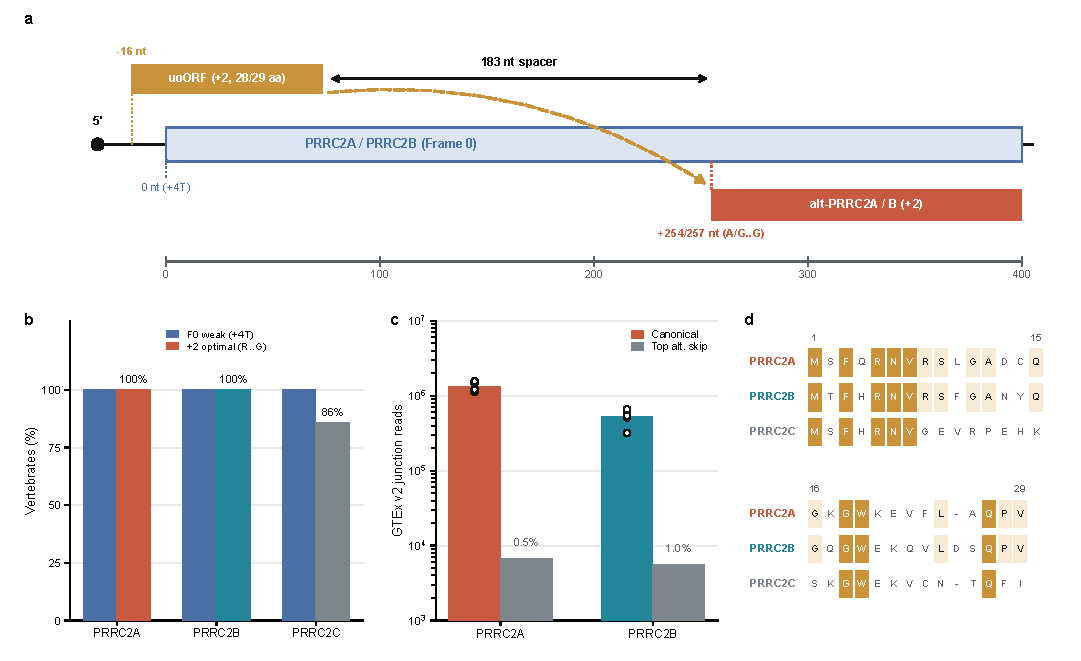
\includegraphics[width=\textwidth]{figures/rendered/fig4.pdf}
  \caption{\textbf{Candidate +2 uoORF reinitiation architecture, 100\%-conserved Kozak asymmetry, and constitutive splicing in \gene{PRRC2A} and \gene{PRRC2B}.} \textbf{a}, To-scale map of the 5' leader and first 400 CDS nucleotides shared by \gene{PRRC2A} and \gene{PRRC2B}. A conserved +2 upstream overlapping ORF (\texttt{uoORF}, ochre) initiates at $-16$\,nt, translates across the suboptimal $+4$\,T Frame-0 start codon (0\,nt, adequate \texttt{G/ATG/T} context), and terminates at \texttt{TGA} (+71/+74\,nt), leaving an exact 183\,nt reinitiation spacer before the optimal \texttt{[A/G]NNATGG} start codon of \gene{alt-PRRC2A/B} (+254/+257\,nt). \textbf{b}, Fraction of 100-way vertebrates retaining the suboptimal $+4$\,T Frame-0 Kozak base (\gene{PRRC2A} 98/98, \gene{PRRC2B} 99/99, \gene{PRRC2C} 100/100; slate blue) versus an optimal purine-at-$-3$ / G-at-$+4$ Kozak context among +2 \texttt{ATG}-bearing vertebrates (colored by paralog: terracotta \gene{PRRC2A} 98/98, petrol teal \gene{PRRC2B} 97/97 [97/98 covered], gray \gene{PRRC2C} degraded to 60/70 [85.7\%; 70/99 covered]). \textbf{c}, Log-scale GTEx v2 Snaptron splice-junction read counts across $\sim 19,000$ human RNA-seq samples comparing mean canonical coding Exon 1--6 internal introns (five symmetric introns per gene; individual introns shown as open circles) against the highest-abundance internal alternative junction (0.5\% and 1.0\% of mean canonical plus alternative reads, gray). \textbf{d}, Sequence alignment of the replicated GENCODE Phase I Ribo-seq +2 uoORF peptides across \gene{PRRC2A} (\texttt{c6riboseqorf41}, 28 aa), \gene{PRRC2B} (\texttt{c9riboseqorf98}, 29 aa), and \gene{PRRC2C} (\texttt{c1riboseqorf224}, 28 aa); solid ochre tiles denote positions invariant across all three paralogs and light ochre tiles denote positions shared between \gene{PRRC2A} and \gene{PRRC2B}.}
  \label{fig:fig4}
\end{figure}

Instead, auditing the 5' leader and GENCODE Phase I ribosome-profiling catalog\refsup{19} uncovered a conserved candidate translational reinitiation architecture across the entire vertebrate \gene{PRRC2} family (Fig.~\ref{fig:fig4}a,b,d). First, although all three human paralogs retain a $-3$ purine at the canonical Frame-0 start codon (giving an adequate/intermediate \texttt{G/ATG/T} context: \texttt{AGCGCAATGTCC} in \gene{PRRC2A}, \texttt{ATCGCAATGTCC} in \gene{PRRC2B}, and \texttt{ACCGAAATGTCG} in \gene{PRRC2C}), every single covered vertebrate in the 100-way alignment preserves a suboptimal pyrimidine (\texttt{T}) at the critical $+4$ Kozak position (98/98 in \gene{PRRC2A}, 99/99 in \gene{PRRC2B}, and 100/100 in \gene{PRRC2C}), whereas the internal +2 start codon of \gene{alt-PRRC2A} (\texttt{A/ATG/G} in 98/98 covered vertebrates) and \gene{alt-PRRC2B} (\texttt{A/ATG/G} in 53/97 and \texttt{G/ATG/G} in 44/97 \texttt{ATG}-bearing vertebrates; 97/98 covered species retain the \texttt{ATG}, 100\% optimal \texttt{R/ATG/G}) maintains a consensus strong Kozak context\refsup{25} (while \gene{PRRC2C} loses the \texttt{ATG} in 29/99 species and relaxes to 85.7\% [60/70] optimal context with \texttt{T}/\texttt{C} leakage among the remaining 70; Fig.~\ref{fig:fig4}b).

Second, and even more remarkably, GENCODE Phase I ribosome profiling independently detects a replicated, actively translated 28--29 aa upstream overlapping ORF (\texttt{uoORF}) on all three human \gene{PRRC2} transcripts: \texttt{c6riboseqorf41} in \gene{PRRC2A} (chr6:31,622,773--31,622,860, 28 aa), \texttt{c9riboseqorf98} in \gene{PRRC2B} (chr9:131,430,128--131,430,218, 29 aa), and \texttt{c1riboseqorf224} in \gene{PRRC2C} (chr1:171,512,072--171,512,159, 28 aa; Fig.~\ref{fig:fig4}d). All three uoORFs are homologous paralogs descended from before the 2R vertebrate duplications (conserving \texttt{M[S/T]F[Q/H]RNV...G[K/Q]GW[K/E]...Q}), and all three initiate at the exact same nucleotide offset---$-16$\,nt upstream of the Frame-0 start codon, in Frame +2. Ribosomes that initiate at this uoORF translate directly past the canonical Frame-0 start codon without recognizing it, terminate at a \texttt{TGA} stop codon at CDS nucleotide 71 (\gene{PRRC2A}) or 74 (\gene{PRRC2B}), and leave an identically sized 183-nucleotide spacer in both \gene{PRRC2A} ($254 - 71 = 183$\,nt) and \gene{PRRC2B} ($257 - 74 = 183$\,nt) before the optimal \texttt{[A/G]NNATGG} start codon of \gene{alt-PRRC2A/B} (Fig.~\ref{fig:fig4}a). This 183\,nt post-termination distance sits squarely inside the classic 150--250\,nt window in which mammalian 40S subunits resume scanning past short-range intervening \texttt{ATG}s (4 in \gene{PRRC2A}, 2 in \gene{PRRC2B}) while reacquiring the eIF2$\cdot$GTP$\cdot$Met-tRNA\textsubscript{i} ternary complex to reinitiate downstream (as established for \gene{ATF4})\refsup{26,27}. Because \gene{PRRC2A}, \gene{PRRC2B}, and \gene{PRRC2C} themselves are the cellular factors that promote leaky scanning past uoORFs\refsup{11,12}, embedding a conserved uoORF-to-\gene{alt-PRRC2} layout inside their own 5' leaders immediately nominates a testable cis-regulatory hypothesis coupling \gene{PRRC2} leaky-scanning activity to the relative output of Frame-0 \gene{PRRC2} versus Frame-+2 \gene{alt-PRRC2}.

\subsection{Clinical variant re-annotation and genomically audited knockout switches enable immediate genetic dissection in human cells}

Because clinical pipelines annotate \gene{PRRC2A} and \gene{PRRC2B} solely in Frame 0, variants falling inside coding exons 2--6 are currently interpreted without awareness of \gene{alt-PRRC2A} or \gene{alt-PRRC2B}. Translating all 45 ClinVar SNVs\refsup{20} falling within the dual-coding spans of \gene{PRRC2A} and \gene{PRRC2B} into Frame +2 revealed 23 variants that alter the \gene{alt-PRRC2A} or \gene{alt-PRRC2B} protein sequence (Fig.~\ref{fig:fig3}d). Notably, one variant classified as ``Benign'' strictly because it is synonymous in Frame 0 (\gene{PRRC2A} \texttt{c.636G>T}, \texttt{p.Gly212=}, ClinVar ID \texttt{3056017}) actually causes a missense substitution in \gene{alt-PRRC2A} (\texttt{p.Ala128Ser}), while 21 Variants of Uncertain Significance (VUS) and 1 unclassified variant simultaneously alter both proteins---including \gene{PRRC2A} \texttt{c.541A>G} (\texttt{p.Lys181Glu} / \gene{alt-PRRC2A} \texttt{p.Gln96Arg}, ID \texttt{2325756}), \texttt{c.547G>T} (\texttt{p.Ala183Ser} / \texttt{p.Cys98Phe}, ID \texttt{2401614}), and \gene{PRRC2B} \texttt{c.496T>A/G} (\texttt{p.Ser166Thr/Ala} / \gene{alt-PRRC2B} \texttt{p.Ile80Asn/Ser}, IDs \texttt{3426163}/\texttt{2218317}) hitting the 500-My conserved \texttt{SRGIS} and \texttt{WRPGQGCQ} cores.

Finally, to enable clean functional dissection of \gene{alt-PRRC2A} and \gene{alt-PRRC2B} in human cell lines without altering a single amino acid of Frame-0 \gene{PRRC2A} or \gene{PRRC2B}, we enumerated all single-nucleotide substitutions across both dual-coding spans that are strictly synonymous in Frame 0 while creating premature stop codons in Frame +2 (22 candidate switches in \gene{PRRC2A} and 20 in \gene{PRRC2B}; Fig.~\ref{fig:fig3}d), and audited every \texttt{C>T} candidate directly against hg38 genomic sequence (including adjacent introns for splice-proximal sites) for canonical \texttt{NGG} or PAM-relaxed \texttt{NG} PAMs across protospacer positions 4--8 and bystander cytosines within $[-3\ldots+3]$ (Table~\ref{tab:switches}). Strikingly, both paralogs carry a matched, completely bystander-free \texttt{Q4*} switch (\gene{PRRC2A} \texttt{c.264C>T} [\texttt{S88S}/\texttt{Q4*}, \texttt{GGCAAG[C]AAACAG}] and \gene{PRRC2B} \texttt{c.267C>T} [\texttt{N89N}/\texttt{Q4*}, \texttt{GGCAAA[C]AAGCAG}]) that truncates \gene{alt-PRRC2A/B} prior to all three conserved motifs (Motif 1 starts at residue 19) with an exact \texttt{NG} PAM (\texttt{CGA}/\texttt{AGA}) placing the target cytosine at protospacer position 6 for PAM-relaxed \texttt{SpCas9-NG}/\texttt{SpRY}-CBE (or prime editing). In addition, both paralogs carry a matched bystander-free canonical \texttt{NGG}-PAM CBE switch (\gene{PRRC2A} \texttt{c.540C>T} [\texttt{D180D}/\texttt{Q96*}, PAM \texttt{GGG}/\texttt{AGG} at pos 4--5] and \gene{PRRC2B} \texttt{c.546C>T} [\texttt{D182D}/\texttt{Q97*}, PAM \texttt{AGG} at pos 4]) that ablates the C-terminal \texttt{VVWARTKPPP} motif, and \gene{PRRC2B} carries a bystander-free \texttt{Q44*} \texttt{SpCas9-NG}-CBE switch (\texttt{c.387C>T}, PAM \texttt{TGC} at pos 6). By contrast, five \texttt{TCC}/\texttt{CCC} switches (\gene{PRRC2A} \texttt{R9*}, \texttt{Q11*}, \texttt{Q35*}; \gene{PRRC2B} \texttt{Q14*}, \texttt{Q35*}, where \texttt{Q35*} lies downstream of Motif 1 and truncates prior to Motifs 2--3) harbor adjacent $-1$/$-2$ cytosine bystanders whose co-editing would cause Frame-0 missense substitutions (\texttt{S93F}, \texttt{P95S/L}, \texttt{S99F}, \texttt{S119F}, \texttt{S120F}) and therefore require prime editing (PE) or narrow-window CBE with clonal allele verification (Table~\ref{tab:switches}).

\begin{table}[!htbp]
\centering
\caption{\textbf{Genomically audited single-nucleotide knockout switches (\texttt{C>T}) in human \gene{PRRC2A} (\texttt{ENST00000376033.3}) and \gene{PRRC2B} (\texttt{ENST00000357304.8}) that truncate \gene{alt-PRRC2A/B} without changing a single amino acid of Frame-0 \gene{PRRC2A/B}.} PAMs (protospacer positions 4--8, including intronic flanks) and $[-3\ldots+3]$ cytosine bystanders were verified directly against hg38 genomic DNA.}
\label{tab:switches}
\footnotesize
\renewcommand{\arraystretch}{1.18}
\resizebox{\textwidth}{!}{%
\begin{tabular}{@{}lllllllll@{}}
\toprule
\textbf{Gene} & \textbf{CDS sub.} & \textbf{hg38 coordinate} & \textbf{Frame-0 (codon; usage/1k)} & \textbf{Frame +2 (codon)} & \textbf{Location in +2} & \textbf{PAM (pos 4--8)} & \textbf{Bystander C ($[-3..+3]$)} & \textbf{Recommended editor} \\
\midrule
\gene{PRRC2A} & \texttt{c.264C>T} & \texttt{chr6:31,623,883} & \texttt{S88S} (\texttt{AGC}$\rightarrow$\texttt{AGT}; 19.5$\rightarrow$12.1) & \texttt{Q4*} (\texttt{CAA}$\rightarrow$\texttt{TAA}) & Pre-Motif 1 (paralog of 2B \texttt{Q4*}) & \texttt{NG}: \texttt{CGA} (p6) & None & \texttt{SpCas9-NG}/\texttt{SpRY}-CBE or PE \\
\gene{PRRC2A} & \texttt{c.279C>T} & \texttt{chr6:31,623,898} & \texttt{S93S} (\texttt{TCC}$\rightarrow$\texttt{TCT}; 17.7$\rightarrow$15.2) & \texttt{R9*} (\texttt{CGA}$\rightarrow$\texttt{TGA}) & Pre-Motif 1 (\texttt{SAAGIA}) & \texttt{NG}: \texttt{AGA} (p7; intron) & \texttt{-1C} (F0 \texttt{S93F}), \texttt{+3C} (syn) & Prime editing (PE) \\
\gene{PRRC2A} & \texttt{c.285C>T} & \texttt{chr6:31,623,904} & \texttt{P95P} (\texttt{CCC}$\rightarrow$\texttt{CCT}; 19.8$\rightarrow$17.5) & \texttt{Q11*} (\texttt{CAA}$\rightarrow$\texttt{TAA}) & Pre-Motif 1 (5\,bp to 3' donor) & \texttt{NGG}: \texttt{AGG} (p7; intron) & \texttt{-2/-1C} (F0 \texttt{P95S/L}), \texttt{-3C} (syn) & Prime editing (PE) \\
\gene{PRRC2A} & \texttt{c.357C>T} & \texttt{chr6:31,624,327} & \texttt{S119S} (\texttt{TCC}$\rightarrow$\texttt{TCT}; 17.7$\rightarrow$15.2) & \texttt{Q35*} (\texttt{CAA}$\rightarrow$\texttt{TAA}) & Post-Motif 1, pre-Motif 2 & \texttt{NG}: \texttt{CGA} (p8) & \texttt{-1C} (F0 \texttt{S119F}), \texttt{-3/+3C} (syn) & Prime editing (PE) \\
\gene{PRRC2A} & \texttt{c.540C>T} & \texttt{chr6:31,625,247} & \texttt{D180D} (\texttt{GAC}$\rightarrow$\texttt{GAT}; 25.1$\rightarrow$21.8) & \texttt{Q96*} (\texttt{CAA}$\rightarrow$\texttt{TAA}) & Pre-\texttt{VVWARTKPPP} (paralog of 2B \texttt{Q97*}) & \texttt{NGG}: \texttt{GGG} (p4), \texttt{AGG} (p5) & None & \texttt{SpCas9-NGG}-CBE (clean) \\
\midrule
\gene{PRRC2B} & \texttt{c.267C>T} & \texttt{chr9:131,432,768} & \texttt{N89N} (\texttt{AAC}$\rightarrow$\texttt{AAT}; 19.1$\rightarrow$17.0) & \texttt{Q4*} (\texttt{CAA}$\rightarrow$\texttt{TAA}) & Pre-Motif 1 (paralog of 2A \texttt{Q4*}) & \texttt{NG}: \texttt{AGA} (p6) & None & \texttt{SpCas9-NG}/\texttt{SpRY}-CBE or PE \\
\gene{PRRC2B} & \texttt{c.297C>T} & \texttt{chr9:131,436,623} & \texttt{S99S} (\texttt{TCC}$\rightarrow$\texttt{TCT}; 17.7$\rightarrow$15.2) & \texttt{Q14*} (\texttt{CAG}$\rightarrow$\texttt{TAG}) & Pre-Motif 1 (3\,bp to 5' acceptor) & \texttt{NG}: \texttt{AGC} (p4) & \texttt{-1C} (F0 \texttt{S99F}) & Prime editing (PE) \\
\gene{PRRC2B} & \texttt{c.360C>T} & \texttt{chr9:131,436,686} & \texttt{S120S} (\texttt{TCC}$\rightarrow$\texttt{TCT}; 17.7$\rightarrow$15.2) & \texttt{Q35*} (\texttt{CAA}$\rightarrow$\texttt{TAA}) & Post-Motif 1, pre-Motif 2 & \texttt{NG}: \texttt{CGA} (p7) & \texttt{-1C} (F0 \texttt{S120F}), \texttt{-3C} (syn) & Prime editing (PE) \\
\gene{PRRC2B} & \texttt{c.387C>T} & \texttt{chr9:131,436,713} & \texttt{I129I} (\texttt{ATC}$\rightarrow$\texttt{ATT}; 20.8$\rightarrow$16.0) & \texttt{Q44*} (\texttt{CAG}$\rightarrow$\texttt{TAG}) & Pre-Motif 2 (\texttt{KGLKPTV}) & \texttt{NG}: \texttt{TGC} (p6; intron) & None & \texttt{SpCas9-NG}/\texttt{SpRY}-CBE or PE \\
\gene{PRRC2B} & \texttt{c.546C>T} & \texttt{chr9:131,444,261} & \texttt{D182D} (\texttt{GAC}$\rightarrow$\texttt{GAT}; 25.1$\rightarrow$21.8) & \texttt{Q97*} (\texttt{CAA}$\rightarrow$\texttt{TAA}) & Pre-\texttt{VVWARTKPPP} (paralog of 2A \texttt{Q96*}) & \texttt{NGG}: \texttt{AGG} (p4) & None & \texttt{SpCas9-NGG}-CBE (clean) \\
\bottomrule
\end{tabular}}
\end{table}

% ============================================================================
% 3. DISCUSSION
% ============================================================================
\section{Discussion}

\subsection{Why the N-terminal BAT2 domain of \gene{PRRC2A} and \gene{PRRC2B} diverged from \gene{PRRC2C}}

Our findings offer a direct evolutionary explanation for an observation that has puzzled recent structural and sequence analyses of the human \gene{PRRC2} family. While the C-terminal coiled-coil and RG-rich regions of \gene{PRRC2A}, \gene{PRRC2B}, and \gene{PRRC2C} share recognizable interactions with eIF3 and stress-granule machinery, their N-terminal $\sim 200$-residue BAT2 region lacks a stable globular fold and exhibits unexpected compositional divergence between \gene{PRRC2C} and \gene{PRRC2A}/\gene{PRRC2B}\refsup{13}. The discovery that coding exons 2--6 of \gene{PRRC2A} and \gene{PRRC2B} have been dual-coding for roughly 580 million years explains both anomalies at once: the disordered Frame-0 BAT2 polypeptide acts as a permissive structural cradle capable of accommodating extreme nucleotide-level constraint imposed by a second protein in Frame +2, while the release of \gene{PRRC2C} from +2 dual-coding constraint before 465\,Mya allowed its BAT2 nucleotide and amino-acid composition to drift freely for nearly half a billion years.

This evolutionary history also makes \gene{PRRC2A}/\gene{PRRC2B} versus \gene{PRRC2C} one of the cleanest natural experiments in human comparative genomics. Because all three paralogs descend from the same ancestral locus and share nearly identical exon-intron boundaries, splice architecture, and uoORF positioning, \gene{PRRC2C} controls simultaneously for locus-specific exon length, 5'-proximal codon usage, and mutational context. Every signature of Frame-+2 selection---strict non-stop-risk 4D elevation ($P \le 3.74 \times 10^{-6}$ versus \gene{PRRC2C}), 5-frame stop-codon purging (0.05--0.08 versus 9.91 stops), +2 amino-acid preservation at host-divergent columns ($P \le 3.14 \times 10^{-5}$), and active purifying selection across 807,162 living humans ($\text{OR} = 0.019$ versus $0.763$)---appears sharply in \gene{PRRC2A} and \gene{PRRC2B} and disappears cleanly in \gene{PRRC2C}.

\subsection{A self-referential translational circuit inside the leaky-scanning regulators}

The architecture of the \gene{PRRC2A} and \gene{PRRC2B} 5' leaders adds an intriguing mechanistic layer to the biology of translational control. \gene{PRRC2A}, \gene{PRRC2B}, and \gene{PRRC2C} were recently identified as dedicated trans-acting regulators that help scanning 43S preinitiation complexes bypass inhibitory uORFs and uoORFs to reach downstream main ORFs\refsup{11,12}. Our audit shows that all three human \gene{PRRC2} mRNAs themselves carry a homologous, actively translated +2 uoORF (\texttt{c6riboseqorf41}, \texttt{c9riboseqorf98}, \texttt{c1riboseqorf224}) starting at $-16$\,nt and terminating 71--74\,nt inside the main CDS, immediately downstream of a 100\%-conserved suboptimal $+4$\,T Frame-0 Kozak sequence (\texttt{G/ATG/T}).

In \gene{PRRC2A} and \gene{PRRC2B}, this uoORF terminates exactly 183 nucleotides upstream of the 100\%-conserved optimal \texttt{[A/G]NNATGG} start codon of \gene{alt-PRRC2A/B}---matching the canonical mammalian reinitiation spacing characterized in \gene{ATF4}\refsup{26,27}. This layout immediately predicts a concrete, testable regulatory switch: when cellular \gene{PRRC2} levels are high (promoting leaky scanning past uoORFs), ribosomes should more readily skip the $-16$\,nt uoORF and access the Frame-0 start codon (or leak past it), whereas when leaky-scanning efficiency drops (or during integrated stress / eIF2$\alpha$ phosphorylation when ternary-complex reacquisition slows), ribosomes translating the uoORF will bypass the Frame-0 start codon and reinitiate downstream at \gene{alt-PRRC2A/B}. Notably, because \gene{PRRC2C} retains the ancestral $-16$\,nt uoORF even after losing \gene{alt-PRRC2}, the uoORF likely serves a dual role across the family: autoregulating Frame-0 \gene{PRRC2} output in all three paralogs while doubling as the dedicated ribosome delivery shuttle for \gene{alt-PRRC2A} and \gene{alt-PRRC2B}.

\subsection{Limitations, open biological questions, and immediate experimental roadmap}

We emphasize clear boundaries between what evolutionary, population-genetic, and transcriptomic evidence establishes and what remains to be determined at the bench. First, our comparative, gnomAD v4.1, PeptideAtlas (\texttt{PE=1} for \texttt{A0A8I5QKQ9}), and GENCODE Ribo-seq findings collectively establish that \gene{alt-PRRC2A} and \gene{alt-PRRC2B} are genuine, translated, 580-My-old human proteins under active purifying selection against both nonsense and missense variation today.

Second, the exact molecular target and biochemical mechanism of \gene{alt-PRRC2A} and \gene{alt-PRRC2B} remain open. Both polypeptides are small (130 and 142 aa), basic, and predicted to be largely intrinsically disordered in isolation, lacking recognizable Pfam or InterPro domains; identifying their physical interactors will require unbiased experimental proximity labeling or endogenous co-immunoprecipitation rather than sequence-based homology alone. Importantly, any prior CRISPR knockout, siRNA knockdown, or coding exon 2--6 deletion experiment targeting \gene{PRRC2A} or \gene{PRRC2B} has simultaneously ablated \gene{alt-PRRC2A} or \gene{alt-PRRC2B}, raising the possibility that a subset of phenotypes attributed to Frame-0 \gene{PRRC2A/B} (or to the chromosome 6 MHC class III \gene{PRRC2A} locus in neurodevelopmental and immune traits) may involve or depend upon the embedded +2 proteins.

Third, our genomically audited knockout switches (Table~\ref{tab:switches}) provide a clean, non-destructive way to decouple Frame 0 from Frame +2 directly in human cells. Introducing \gene{PRRC2A} \texttt{c.264C>T} (\texttt{S88S}/\texttt{Q4*}) and \gene{PRRC2B} \texttt{c.267C>T} (\texttt{N89N}/\texttt{Q4*}) via bystander-free \texttt{SpCas9-NG}/\texttt{SpRY}-CBE or prime editing (or \texttt{c.540C>T} [\texttt{Q96*}] / \texttt{c.546C>T} [\texttt{Q97*}] via canonical \texttt{SpCas9-NGG}-CBE)---individually and in double-knockout combination to account for paralog redundancy---together with C-terminal epitope tagging of the endogenous +2 frame and dual-luciferase reporters mutating the $-16$\,nt uoORF start and 183\,nt spacer will directly test (i) uoORF-dependent reinitiation of \gene{alt-PRRC2A/B} under basal and stress conditions, (ii) endogenous protein localization and binding partners, and (iii) whether loss of \gene{alt-PRRC2A/B} perturbs cellular leaky scanning, stress-granule dynamics, or cell fitness independently of Frame-0 \gene{PRRC2A/B}. Finally, assigning official HGNC gene symbols and incorporating \gene{alt-PRRC2A} and \gene{alt-PRRC2B} into RefSeq, GTEx, and clinical variant-interpretation pipelines (VEP/ClinVar) will ensure that Frame-0-silent or VUS alleles disrupting these constrained human proteins are no longer overlooked.

% ============================================================================
% 4. MATERIALS AND METHODS
% ============================================================================
\newpage
\section{Materials and Methods}

\subsection{Genome-wide 100-vertebrate dual-coding screen and database audit}

Canonical human coding exon alignments across 100 vertebrates (\texttt{knownCanonical.exonNuc.fa.gz}, hg38, $n = 23,183$ canonical transcripts) and cross-reference tables (\texttt{kgXref.txt.gz}) were obtained from the UCSC Genome Browser\refsup{28}. Every canonical transcript was translated in Frames +1 and +2 across a balanced 32-vertebrate panel to identify internal stop-free spans ($\ge 50$ codons in human) conserved across vertebrate clades with localized excess fourfold degenerate (4D) synonymous-site identity inside versus outside the candidate interval. Surviving multi-exon candidates were audited against GENCODE v46\refsup{21}, UniProtKB\refsup{22} (\texttt{A0A8I5QKQ9} and \texttt{A0A8I5KXM2}), Ensembl Compara (\texttt{ENSG00000289282} and \texttt{ENSG00000288841}), PeptideAtlas\refsup{23,24}, MMseqs2 against UniRef100\refsup{29}, InterPro/Pfam\refsup{30}, HGNC, NCBI Gene/RefSeq, GTEx, PubMed, Europe PMC, and bioRxiv.

\subsection{Deep metazoan evolutionary tracing}

Orthologous \gene{PRRC2}/\gene{nocte} coding nucleotide sequences containing the N-terminal BAT2 domain (InterPro IPR009738) were retrieved from NCBI RefSeq across protostomes (\spname{Drosophila melanogaster} \texttt{NP\_001245614.1}), hemichordates (\spname{Saccoglossus kowalevskii} \texttt{XP\_077866102.1}), echinoderms (\spname{Strongylocentrotus purpuratus} \texttt{XP\_030852947.1}), cephalochordates (\spname{Branchiostoma floridae} \texttt{XP\_035683835.1}), jawless vertebrates (\spname{Petromyzon marinus} \texttt{XP\_032802661.2}), and cartilaginous fish (\spname{Callorhinchus milii} \gene{prrc2b} \texttt{XM\_042337680.1} and \gene{prrc2c} \texttt{XM\_042335521.1}), bundled in \texttt{data/metazoan\_prrc2\_cds.fa}, and dynamically translated in all three forward reading frames across the homologous BAT2 core to score internal stop counts and conserved sequence motifs. Candidate teleost/sturgeon BAT2--+2 fusion entries (\texttt{A0A444UTE8}/\texttt{RXM91444.1} and \texttt{A0A3B3D8N8}/\texttt{ENSOMET00000004379}) were audited directly at the exon-coordinate level via Ensembl REST and NCBI GenPept records.

\subsection{Vertebrate non-stop-risk 4D selection, 5-frame stop-codon purging, and +2 amino-acid preservation}

Comparative selection analyses were performed on a non-redundant 32-vertebrate reference panel (\texttt{PANEL\_32}, spanning primates, rodents, carnivores, ungulates, marsupials, monotremes, birds, reptiles, amphibians, coelacanth, spotted gar, and teleosts; coverage filter $< 55\%$ alignment gaps across the full CDS, yielding $n = 22$ species for \gene{PRRC2A}, $n = 26$ for \gene{PRRC2B}, and $n = 26$ for \gene{PRRC2C}) as well as the full 100-way alignment for stop-free census and Kozak conservation. Strict non-stop-risk 4D synonymous conservation was evaluated exclusively at aligned Frame-0 4D codons (\texttt{CTN}, \texttt{GTN}, \texttt{TCN}, \texttt{CCN}, \texttt{ACN}, \texttt{GCN}, \texttt{CGN}, \texttt{GGN}) whose third nucleotide cannot create a Frame +2 stop codon (\texttt{TAA}/\texttt{TAG}/\texttt{TGA}) in either human or the aligned vertebrate (i.e., the immediately following Frame-0 codon does not begin with \texttt{AA}, \texttt{AG}, or \texttt{GA}). Sliding-window profiles were computed in 25-codon bins across codons 0--375 with species-level standard errors; paired inside-versus-outside significance was assessed via exact paired Wilcoxon signed-rank tests (\texttt{method="exact"}, one observation per vertebrate species, plus a phylogenetic sensitivity check collapsing species into 8 independent major vertebrate clades), and direct paralog contrasts (\gene{PRRC2A} and \gene{PRRC2B} versus \gene{PRRC2C}) were evaluated via Mann--Whitney $U$ tests.

For the 5-frame stop-codon test ($+1$, $+2$, $-0$, $-1$, $-2$) across the homologous dual-coding span (1-based inclusive Frame-0 codons 85--214 in \gene{PRRC2A}, 86--227 in \gene{PRRC2B}, and 83--216 in \gene{PRRC2C}; $< 15\%$ local gaps, $n = 22$, $25$, and $22$ species), observed stop counts in every species were compared both within-gene against all four other alternative frames (paired Wilcoxon \texttt{method="approx"} for discrete tied integer counts) and against a species-specific within-gene flanking-codon synonymous null (300 replicates per vertebrate; 1,000 replicates for hg38; exact paired Wilcoxon) that resamples Frame-0 synonymous codons inside the overlap strictly from each species' own non-overlapping flanking codons outside $[\text{start}-10\ldots\text{end}+10]$, preserving exact Frame-0 amino-acid sequence and gene-specific codon usage, supplemented by a 1,000-replicate within-window codon-bag synonymous permutation on hg38 holding exact local GC3 and codon composition constant. Direct +2 amino-acid preservation was measured as the fraction of alignment columns inside the overlap where the Frame-0 amino acid diverged from human while the exact overlapping +2 codon(s) containing the actually mutated nucleotide position(s) encoded the identical amino acid(s) to human (requiring $\ge 10$ divergent sites per species; corroborated by checking the upstream $[\text{prev\_b2}, \text{b0}, \text{b1}]$ +2 codon), compared against \gene{PRRC2C} via Mann--Whitney $U$ tests.

\subsection{Mutation-class-stratified gnomAD v4.1 purifying selection and ClinVar / editing-switch mapping}

All exome and genome variants spanning the dual-coding exons of \gene{PRRC2A} (chr6:31,623,730--31,626,100), \gene{PRRC2B} (chr9:131,432,600--131,446,700), and \gene{PRRC2C} (chr1:171,513,001--171,517,814) plus gene-level pLI/LOEUF constraints and QC \texttt{filters} were retrieved from gnomAD v4.1 (\url{https://gnomad.broadinstitute.org})\refsup{14,15} via its GraphQL API and filtered strictly to QC-PASS variants (\texttt{exome.filters == []} or \texttt{genome.filters == []}; 100\% hg38 reference-base concordance across 503/503 coding SNVs in \gene{PRRC2A}, 412/412 in \gene{PRRC2B}, and 385/385 in \gene{PRRC2C}; removing 2, 1, and 3 \texttt{AS\_VQSR} QC-FAIL SNVs inside the respective +2 spans). Every possible SNV within the internal +2 coding span (excluding the +2 start codon in \gene{PRRC2A/B} and existing +2 reference stops in \gene{PRRC2C}) was classified simultaneously by mutational class (\texttt{CpG\_Ti}: \texttt{CpG C>T} or \texttt{G>A}; \texttt{nonCpG\_Ti}: all other transitions; \texttt{Tv}: transversions), Frame-0 consequence, and Frame-+2 consequence; a sensitivity analysis additionally excluded all $\pm 2$\,bp exon-boundary positions to rule out splice-site or spliced-CDS CpG edge effects. Within-stratum comparisons used exact Fisher tests (both one-sided and two-sided reported), and three-stratum summaries used exact hypergeometric-convolution Cochran--Mantel--Haenszel (CMH) tests across \texttt{CpG\_Ti}, \texttt{nonCpG\_Ti}, and \texttt{Tv} alongside unadjusted Mantel--Haenszel common odds ratios. For the Fig.~\ref{fig:fig3}c forest plot, point estimates and 95\% confidence intervals were computed directly as exact conditional maximum-likelihood common odds ratios and exact conditional 95\% confidence intervals from the convolved noncentral hypergeometric distributions (eliminating continuity adjustments for zero-count strata).

Human splice-junction read support across $\sim 19,000$ GTEx v2 RNA-seq samples was queried via Snaptron\refsup{18} (bundled in \texttt{data/gtex\_v2\_snaptron\_junctions.json} with exact coordinates for all five symmetric canonical introns spanning coding exons 1--6 in both paralogs), and translated upstream ORFs were extracted from the GENCODE Phase I Ribo-seq ORF catalog\refsup{19} (file \texttt{GENCODE\_Riboseq\_ORFs.bed}, hg38). ClinVar variants\refsup{20} overlapping \gene{PRRC2A} and \gene{PRRC2B} coding exons 2--6 were retrieved via NCBI E-utilities and mapped directly onto Frame 0 and Frame +2. Single-nucleotide knockout switches were prioritized by strict Frame-0 synonymy, Frame-+2 premature stop generation, human Kazusa codon usage, and direct hg38 genomic sequence verification (including intronic flanks, bundled in \texttt{data/hg38\_prrc2\_switch\_flanks.json}) for \texttt{NGG}/\texttt{NG} PAM placement across protospacer positions 4--8 and $[-3\ldots+3]$ cytosine bystander consequences.

\subsection{Data availability and competing interests}

All multi-panel figures (Graphical Abstract and Figures 1--4) were generated programmatically from verified processed datasets using Matplotlib and Fignimble. All self-contained analysis scripts, compact raw alignment, metazoan CDS, hg38 flank, GTEx v2 Snaptron, and QC-PASS gnomAD v4.1 subsets, ClinVar and knockout switch tables, Fignimble figure scripts, and the compiled preprint are publicly available at \url{https://github.com/koppikarp/prrc2-plus2-dualcoding}. The author declares no competing interests.

% ============================================================================
% REFERENCES (Nature numbered style; 100% verified DOIs)
% ============================================================================
\vspace{4pt}
\section*{References}
\addcontentsline{toc}{section}{References}
{\footnotesize\linespread{0.97}\selectfont\sloppy\interlinepenalty=10000
\begin{enumerate}[leftmargin=1.9em,itemsep=-0.4pt,parsep=0pt,topsep=0.5pt]
  \item Barrell, B. G., Air, G. M. \& Hutchison, C. A. 3rd. Overlapping genes in bacteriophage $\phi$X174. \textit{Nature} \textbf{264}, 34--41 (1976). \url{https://doi.org/10.1038/264034a0}
  \item Wright, B. W., Molloy, M. P. \& Jaschke, P. R. Overlapping genes in natural and engineered genomes. \textit{Nat. Rev. Genet.} \textbf{23}, 154--168 (2022). \url{https://doi.org/10.1038/s41576-021-00417-w}
  \item Quelle, D. E., Zindy, F., Ashmun, R. A. \& Sherr, C. J. Alternative reading frames of the INK4a tumor suppressor gene encode two unrelated proteins capable of inducing cell cycle arrest. \textit{Cell} \textbf{83}, 993--1000 (1995). \url{https://doi.org/10.1016/0092-8674(95)90214-7}
  \item Klemke, M., Kehlenbach, R. H. \& Huttner, W. B. Two overlapping reading frames in a single exon encode interacting proteins---a novel way of gene usage. \textit{EMBO J.} \textbf{20}, 3849--3860 (2001). \url{https://doi.org/10.1093/emboj/20.14.3849}
  \item Bergeron, D. \textit{et al.} An out-of-frame overlapping reading frame in the ataxin-1 coding sequence encodes a novel ataxin-1 interacting protein. \textit{J. Biol. Chem.} \textbf{288}, 21824--21835 (2013). \url{https://doi.org/10.1074/jbc.M113.472654}
  \item Loughran, G. \textit{et al.} Unusually efficient CUG initiation of an overlapping reading frame in \gene{POLG} mRNA yields novel protein POLGARF. \textit{Proc. Natl. Acad. Sci. U.S.A.} \textbf{117}, 24936--24946 (2020). \url{https://doi.org/10.1073/pnas.2001433117}
  \item Brunet, M. A. \textit{et al.} The \gene{FUS} gene is dual-coding with both proteins contributing to FUS-mediated toxicity. \textit{EMBO Rep.} \textbf{22}, e50640 (2021). \url{https://doi.org/10.15252/embr.202050640}
  \item Cao, X. \textit{et al.} Alt-RPL36 downregulates the PI3K-AKT-mTOR signaling pathway by interacting with TMEM24. \textit{Nat. Commun.} \textbf{12}, 508 (2021). \url{https://doi.org/10.1038/s41467-020-20841-6}
  \item Lin, M. F., Jungreis, I. \& Kellis, M. PhyloCSF: a comparative genomics method to distinguish protein coding and non-coding regions. \textit{Bioinformatics} \textbf{27}, i275--i282 (2011). \url{https://doi.org/10.1093/bioinformatics/btr209}
  \item Orr, M. W., Mao, Y., Storz, G. \& Qian, S.-B. Alternative ORFs and small ORFs: shedding light on the dark proteome. \textit{Nucleic Acids Res.} \textbf{48}, 1029--1042 (2020). \url{https://doi.org/10.1093/nar/gkz734}
  \item Bohlen, J., Roiuk, M., Neff, M. \& Teleman, A. A. PRRC2 proteins impact translation initiation by promoting leaky scanning. \textit{Nucleic Acids Res.} \textbf{51}, 3391--3409 (2023). \url{https://doi.org/10.1093/nar/gkad135}
  \item Jiang, F. \textit{et al.} RNA-binding protein PRRC2B mediates translation of specific mRNAs and regulates cell cycle progression. \textit{Nucleic Acids Res.} \textbf{51}, 5831--5846 (2023). \url{https://doi.org/10.1093/nar/gkad322}
  \item Huang, J. Q. \textit{et al.} PRRC2A, PRRC2B and PRRC2C are stress granule proteins that promote translation through association with the eIF3 complex. Preprint at \textit{bioRxiv} \url{https://doi.org/10.64898/2026.02.24.707808} (2026).
  \item Karczewski, K. J. \textit{et al.} The mutational constraint spectrum quantified from variation in 141,456 humans. \textit{Nature} \textbf{581}, 434--443 (2020). \url{https://doi.org/10.1038/s41586-020-2308-7}
  \item Chen, S. \textit{et al.} A genomic mutational constraint map using variation in 76,156 human genomes. \textit{Nature} \textbf{625}, 92--100 (2024). \url{https://doi.org/10.1038/s41586-023-06045-0}
  \item Wu, R. \textit{et al.} A novel m$^6$A reader Prrc2a controls oligodendroglial specification and myelination. \textit{Cell Res.} \textbf{29}, 23--41 (2019). \url{https://doi.org/10.1038/s41422-018-0113-8}
  \item Sehadova, H. \textit{et al.} Temperature entrainment of \spname{Drosophila}'s circadian clock involves the gene \gene{nocte} and signaling from peripheral sensory tissues to the brain. \textit{Neuron} \textbf{64}, 251--266 (2009). \url{https://doi.org/10.1016/j.neuron.2009.08.026}
  \item Wilks, C. \textit{et al.} Snaptron: querying splicing patterns across tens of thousands of RNA-seq samples. \textit{Bioinformatics} \textbf{34}, 114--116 (2018). \url{https://doi.org/10.1093/bioinformatics/btx547}
  \item Mudge, J. M. \textit{et al.} Standardized annotation of translated open reading frames. \textit{Nat. Biotechnol.} \textbf{40}, 994--999 (2022). \url{https://doi.org/10.1038/s41587-022-01369-0}
  \item Landrum, M. J. \textit{et al.} ClinVar: improvements to accessing data. \textit{Nucleic Acids Res.} \textbf{48}, D835--D844 (2020). \url{https://doi.org/10.1093/nar/gkz972}
  \item Frankish, A. \textit{et al.} GENCODE: reference annotation for the human and mouse genomes in 2023. \textit{Nucleic Acids Res.} \textbf{51}, D942--D949 (2023). \url{https://doi.org/10.1093/nar/gkac1071}
  \item UniProt Consortium. UniProt: the Universal Protein Knowledgebase in 2025. \textit{Nucleic Acids Res.} \textbf{53}, D609--D617 (2025). \url{https://doi.org/10.1093/nar/gkae1010}
  \item Desiere, F. \textit{et al.} The PeptideAtlas project. \textit{Nucleic Acids Res.} \textbf{34}, D655--D658 (2006). \url{https://doi.org/10.1093/nar/gkj040}
  \item Deutsch, E. W. \textit{et al.} The ProteomeXchange consortium at 10 years: 2023 update. \textit{Nucleic Acids Res.} \textbf{51}, D1539--D1548 (2023). \url{https://doi.org/10.1093/nar/gkac1040}
  \item Kozak, M. Point mutations define a sequence flanking the AUG initiator codon that modulates translation by eukaryotic ribosomes. \textit{Cell} \textbf{44}, 283--292 (1986). \url{https://doi.org/10.1016/0092-8674(86)90762-2}
  \item Vattem, K. M. \& Wek, R. C. Reinitiation involving upstream ORFs regulates ATF4 mRNA translation in mammalian cells. \textit{Proc. Natl. Acad. Sci. U.S.A.} \textbf{101}, 11269--11274 (2004). \url{https://doi.org/10.1073/pnas.0400541101}
  \item Hinnebusch, A. G., Ivanov, I. P. \& Sonenberg, N. Translational control by 5'-untranslated regions of eukaryotic mRNAs. \textit{Science} \textbf{352}, 1413--1416 (2016). \url{https://doi.org/10.1126/science.aad9868}
  \item Nassar, L. R. \textit{et al.} The UCSC Genome Browser database: 2023 update. \textit{Nucleic Acids Res.} \textbf{51}, D1188--D1195 (2023). \url{https://doi.org/10.1093/nar/gkac1072}
  \item Steinegger, M. \& S\"oding, J. MMseqs2 enables sensitive protein sequence searching for the analysis of massive data sets. \textit{Nat. Biotechnol.} \textbf{35}, 1026--1028 (2017). \url{https://doi.org/10.1038/nbt.3988}
  \item Blum, M. \textit{et al.} InterPro: the protein sequence classification resource in 2025. \textit{Nucleic Acids Res.} \textbf{53}, D444--D456 (2025). \url{https://doi.org/10.1093/nar/gkae1082}
\end{enumerate}
}

\end{document}
